%! TEX program = xelatex
%! TEX encoding = UTF-8 Unicode

\documentclass[engineeringmaster]{hquThesis}
\usepackage{lineno}
\usepackage{amsmath,amsfonts,amssymb,textcomp}
\usepackage{booktabs,multirow,tabularx,float}
\hypersetup{colorlinks=true,linkcolor=black,citecolor=black}
\begin{document}
\makecover
% NOTE: 正式文档请取消下面两行注释
% {
    \begin{center}
        \sffamily\fontsize{16pt}{25pt}\selectfont 学\hspace{8pt}位\hspace{8pt}论\hspace{8pt}文\hspace{8pt}答\hspace{8pt}辩\hspace{8pt}委\hspace{8pt}员\hspace{8pt}会\hspace{8pt}决\hspace{8pt}议
    \end{center}
} \vspace{32pt}
{
    \fontsize{14pt}{26pt}\selectfont
    \noindent\hspace{28pt}\rmfamily 根据《中华人民共和国学位条例》、《中华人民共和国学位条例暂行实 施办法》、《华侨大学学位授予工作细则》及《华侨大学研究生学位论文质 量监控与评阅答辩的管理规定》的规定,学位论文答辩委员会经充分交换意 见,对论文做出评价,并以无记名投票方式进行表决,同意该同学通过\degree 学位论文答辩,同意授予\degree 学位。\par
    \vspace{192pt}
    \noindent\flushright 答辩委员会(主席签字):\underline{\hspace{156pt}}\vspace{14pt} \par
    \noindent\flushright 答辩时间:\underline{\hspace{60pt}}年\underline{\hspace{25pt}}月\underline{\hspace{25pt}}日 \par
}

% \noindent\fbox{%
    \parbox{14.3cm}{
    \vspace{24pt}\begin{center}\sffamily\fontsize{16pt}{\baselineskip}\selectfont 学位论文独创性声明\end{center}\vspace{18pt}
    \hspace{28pt}\declarationfont\fontsize{14pt}{28pt}\selectfont
    本人声明兹呈交的学位论文是本人在导师指导下完成的研究成果。论文写作中不包含其他人已经发表或撰写过的研究内容,如参考他人或集体的科研成果,均在论文中以明确的方式说明。本人依法享有和承担由此论文所产生的权利和责任。\par
    \vspace{28pt}\hspace{28pt} 论文作者签名:\underline{\hspace{112pt}}\hspace{7pt}签名日期:\underline{\hspace{77pt}}\par\vspace{7pt}
    }%
}
\par
\vspace{44pt}
\noindent\framebox[\linewidth]{
    \parbox{14.3cm}{
    \vspace{24pt}\begin{center}\sffamily\fontsize{16pt}{\baselineskip}\selectfont 学位论文版权使用授权声明\par\end{center}\vspace{18pt}
    \hspace{28pt}\declarationfont\fontsize{14pt}{28pt}\selectfont 
    本人同意授权华侨大学有权保留并向国家机关或机构送交学位论文的复印件和电子版,允许学位论文被查阅和借阅。本人授权华侨大学可以将本学位论文的全部内容或部分内容编入有关数据库进行检索,可以采用影印、缩印或扫描等复制手段保存和汇编本学位论文。\par\vspace{28pt}
    \hspace{28pt}论文作者签名:\underline{\hspace{84pt}}\hspace{7pt}指导老师签名:\underline{\hspace{84pt}}\par
    \hspace{28pt}签\hspace{7pt}名\hspace{7pt}日\hspace{7pt}期:\underline{\hspace{91pt}}\hspace{7pt}签\hspace{7pt}名\hspace{7pt}日\hspace{7pt}期:\underline{\hspace{91pt}}\par\vspace{7pt}
    }
}


\frontmatter{
    
\begin{abstract}
自锁问题是有限元分析中的一类常见数值问题,主要表现为在模拟某些特定物理现象时,数值解因过度约束而丧失精度或收敛性。
常见的自锁问题包括以下两类:体积自锁:在模拟不可压缩材料时,由于体积应变能的过度约束,导致数值解出现刚化现象,无法准确描述材料的变形特性;剪切自锁:在模拟中厚板结构时,由于剪切应变能的过度约束,导致数值解无法准确反映结构的实际变形行为。
混合有限元法是解决自锁问题的常用方法,通过引入额外的场变量(如压力场)来减少过度约束。
例如,在不可压问题中,使用位移--压力混合离散可以有效缓解体积自锁现象。
然而,混合有限元法必须满足LBB稳定性条件,才能保证数值解的稳定性,在一定情况下也可能会产生压力振荡现象。因此,选择合适的变量间约束比至关重要。
尽管混合有限元法常用于解决自锁问题,但并非所有混合离散方案都满足LBB稳定性条件,而已知的满足LBB稳定性条件的混合离散方案常常表现出过度约束的状态。
无网格法具有不依赖于几何拓扑关系的高阶光滑形函数,能够任意的布置节点,特别适用于变量间的混合离散过程。通过结合无网格法与混合有限元法,可以有效解决传统方法中的问题。

本文针对传统混合离散方案存在的问题,提出了一种有限元无网格混合离散分析方法。
并在该方法的基础上,研究了体积不可压问题和中厚板剪切自锁问题中离散节点分布与LBB稳定性条件之间的关系,建立了考虑最优约束比的LBB稳定性条件验证方法,从而确定免自锁的最优约束比范围。
依托再生核无网格法理论框架,通过调整约束比,生成了一种免自锁且满足LBB稳定性条件的有限元无网格混合离散方案。
最后,通过体积不可压问题和中厚板问题的系列经典算例,验证了所提LBB稳定性条件验证方法的正确性,以及有限元无网格混合离散方案的计算精度和稳定性。

\end{abstract}
\keywords{自锁问题;混合离散;最优约束比;LBB稳定性条件;无网格法}

\begin{abstractEn}
Locking problems are a common class of numerical issues in finite element analysis, primarily manifested as a loss of accuracy or convergence in numerical solutions due to excessive constraints when simulating specific physical phenomena. 
Typical locking problems include two categories: volumetric locking, where numerical solutions exhibit artificial stiffening due to over-constrained volumetric strain energy in modeling incompressible materials, and shear locking, where numerical solutions fail to accurately reflect the deformation behavior of moderately thick plate structures due to over-constrained shear strain energy. 
The mixed finite element method is widely used to address locking problems by introducing additional field variables (e.g., pressure fields) to relax excessive constraints. For instance, displacement-pressure mixed discretization effectively mitigates volumetric locking in incompressible problems. 
However, the mixed finite element method must satisfy the LBB (Ladyzhenskaya-Babuška-Brezzi) stability conditions to ensure numerical stability, and pressure oscillations may still occur under certain circumstances. 
Therefore, selecting an appropriate constraint ratio between variables is critical. Although the mixed finite element method is commonly employed to resolve locking problems, not all mixed discretization schemes satisfy the LBB stability conditions. Even known LBB-compliant schemes often exhibit over-constrained states.
Meshfree methods, characterized by high-order smooth shape functions independent of geometric topology and flexible node arrangement, are particularly suitable for mixed discretization processes involving multiple variables. By integrating meshfree methods with the mixed finite element approach, traditional limitations can be effectively addressed.

This study proposes a finite element-meshfree hybrid discretization method to tackle the shortcomings of conventional mixed discretization schemes. 
Building on this method, the relationship between discrete node distributions and LBB stability conditions is systematically investigated for both incompressible problems and moderately thick plate shear locking problems.
A verification framework for LBB stability conditions incorporating an optimal constraint ratio is established to determine the optimal constraint range for locking-free solutions. 
Leveraging the theoretical framework of the reproducing kernel meshfree method, a locking-free hybrid discretization scheme satisfying LBB stability conditions is developed by adjusting the constraint ratio. 
Finally, a series of benchmark cases for incompressible problems and moderately thick plate problems validate the correctness of the proposed LBB stability verification framework and demonstrate the computational accuracy and stability of the finite element-meshfree hybrid discretization scheme.

\end{abstractEn}
\keywordsEn{Locking problems; Mixed discretization;  Optimal constraint ratio;LBB stability conditions; Meshfree method}

    \tableofcontents
}

\mainmatter
\chapter{前期准备}
\section{封面关键字设置}
\section{Git相关}
使用fork建仓

同步文件选择,不同步编译文件(*.aux, *.fls, *.log ……)

\section{VS code配置}
LaTeX workshop: 快捷键,搜索(forward research)与反向搜索(inverse research)。

Git Graph: 查看修改(diff)

Todo Tree: magic comment

% TODO: add magic comment
LaTeX: magic comment

Zotero LaTeX:Zotero管理参考文献
\section{文件、label 命名规则}
公式:label\{chapter\{name\}-formula1-name\}

图:label\{chapter\{name\}-fig1-name\}

表:label\{chapter\{name\}-table1-name\}

\chapter{图表设置}
单张
\begin{figure}[H]
    \centering
    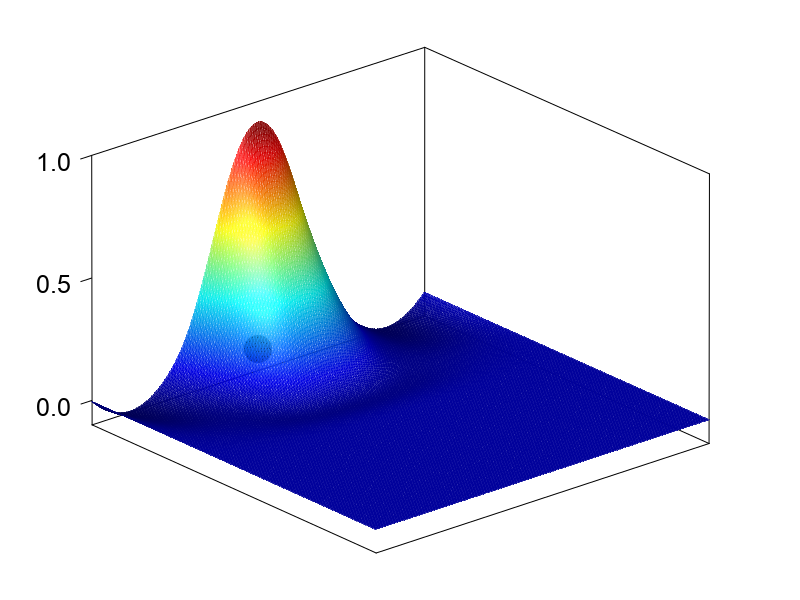
\includegraphics[scale=0.4]{figure/1.png}
\caption{\centering{边界点处无网格形函数}}
\label{chapter-Graphsettings-fig1-meshfree}
\end{figure}

并排
\begin{figure}[H]
    \centering
    \begin{subcaptiongroup}
    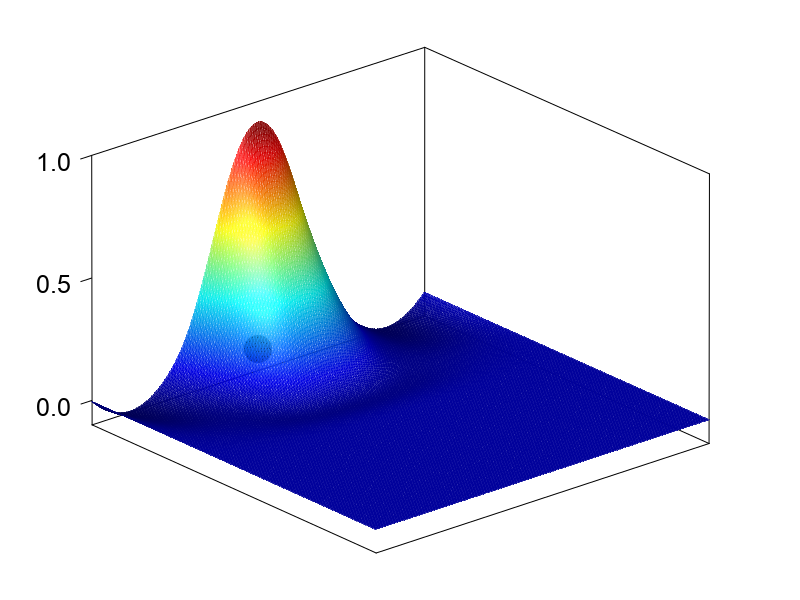
\includegraphics[width=0.49\textwidth]{figure/1.png}
    \phantomcaption\label{1}
    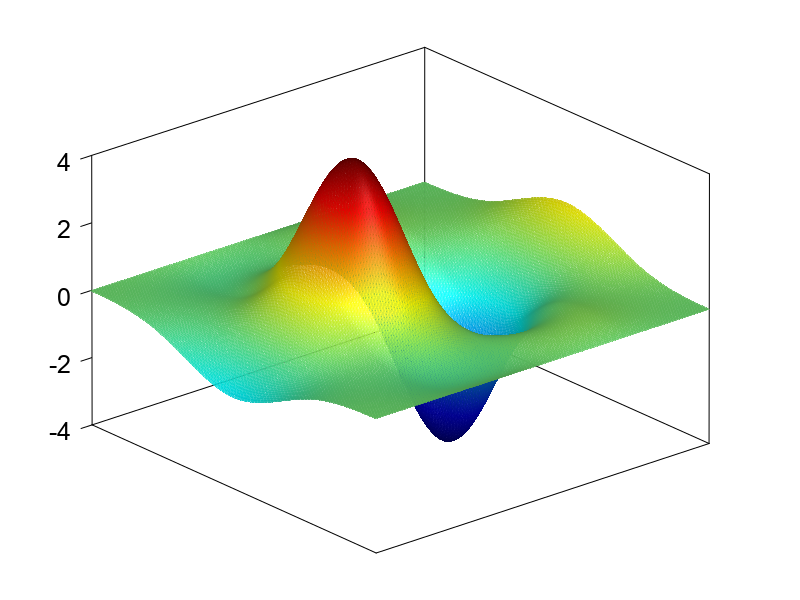
\includegraphics[width=0.49\textwidth]{figure/2.png}
    \phantomcaption\label{2}
    \end{subcaptiongroup}
\caption{\centering{无网格形函数:\subref{1}边界点;\subref{2}中心点}}

% 遇到图名过长需要换行的编写:
% \caption{\centering{标题:\protect\linebreak \subref{xxx} 小标题1;\subref{xx} 小标题2;\subref{xxx}小标题3;\subref{xxx} 小标题4}}

\label{chapter-Graphsettings-fig2-meshfree}
\end{figure}
图\ref{chapter-Graphsettings-fig1-meshfree}、\ref{chapter-Graphsettings-fig2-meshfree}分别表示边界点处和内部节点处的无网格形函数图。

\newpage


三线表
\begin{table}[H]
    \caption{\textbf{三次基函数无网格法分片实验结果}}
    \centering\label{chapter-table-cubic}
    \begin{tabular}{lcccc}
       \toprule
    & \multicolumn{2}{c}{二次分片实验} & \multicolumn{2}{c}{三次分片实验} \\ \cline{2-5}
       &$L_2$-Error$\quad$&$H_1$-Error&$L_2$-Error$\quad$&$H_1$-Error\\
       \midrule
      RKGSI-Penalty&$1.4\times10^{-7}$&$2.1\times10^{-6}$&$2.0\times10^{-7}$&$2.7\times10^{-6}$\\
      RKGSI-LM&$3.0\times10^{-4}$&$9.8\times10^{-3}$&$4.2\times10^{-4}$&$9.8\times10^{-3}$\\
      RKGSI-Nitsche&$3.6\times10^{-15}$&$1.0\times10^{-13}$&$4.6\times10^{-15}$&$9.5\times10^{-14}$\\
      RKGSI-HR&$3.1\times10^{-15}$&$1.0\times10^{-13}$&$3.5\times10^{-15}$&$7.4\times10^{-14}$\\
       \bottomrule
    \end{tabular}
    \end{table}
表\ref{chapter-table-cubic}为三次基函数无网格法的分片试验结果。


\chapter{使用Zotero管理参考文献}
添加附件:Better BibTex

建立文件库:references

对文件库导出条目至Latex编写的文件夹路径中(Latex路径中只允许以英文命名)

eg:基于赫林格-赖斯纳原理的变分一致型伽辽金无网格法\cite{Wu2022,wu2023}相较于传统的本质边界条件施加方法能够有效提高计算精度和计算效率。




\chapter{\LaTeX 插件推荐}
编写公式、图表可能需要用到的包:

usepackage\{amsmath,amsfonts,amssymb,textcomp\}

usepackage\{booktabs,multirow,tabularx,float\}

\begin{acknowledgements}
感谢
\end{acknowledgements}


\appendix

\chapter{附录}
本附录描述的是....


\backmatter
\bibliography{references}
\begin{cv}
    \section*{个人简历}
    XXX,女,汉族,XXXX年XX月XX日出生,XX省XXX人。

    XXXX年XX月毕业于XXXX学校XXXX专业,获得工学学士学位。

    XXXX年XX月至今就读于华侨大学土木工程学院土木水利专业,攻读工学硕士学位。
    \section*{在学期间发表的论文}
    \begin{enumerate}[{[1]}]
        \item 吴俊超, 邓俊俊, 王家睿, 等. 伽辽金型无网格法的数值积分方法[J]. 固体力学学报, 2016, 3(37): 208-233. 
        \item 吴俊超, 邓俊俊, 王家睿, 等. 伽辽金型无网格法的数值积分方法[J]. 固体力学学报, 2016, 3(37): 208-233. 
    \end{enumerate}
\end{cv}


\end{document}
